\documentclass[a4paper,10pt]{article}
\usepackage{graphicx}
\usepackage{caption}
\usepackage{enumitem}
\usepackage{multicol}
\usepackage{mathtools}
\usepackage{amsmath,amsthm,amssymb,cancel,bm}
\usepackage{floatrow}
\setcounter{tocdepth}{2}
\usepackage{geometry}
\geometry{total={210mm,297mm},
left=25mm,right=25mm,%
bindingoffset=0mm, top=20mm,bottom=20mm}
\newcommand{\linia}{\rule{\linewidth}{0.5pt}}
\AtBeginDocument{%
   \setlength\abovedisplayskip{-3pt}
   \setlength\belowdisplayskip{5pt}}

\usepackage{hyperref}
\hypersetup{colorlinks=true,linkcolor=blue,citecolor=green,filecolor=cyan,urlcolor=magenta}

% my own titles
\makeatletter
\renewcommand{\maketitle}{
\begin{center}
\vspace{2ex}
{\huge \textsc{\@title}}
\vspace{1ex}
\\
\linia\\
\@author
\vspace{4ex}
\end{center}
}
\makeatother

% custom footers and headers
\usepackage{fancyhdr,lastpage}
\pagestyle{fancy}
\lhead{}
\chead{}
\rhead{}
\renewcommand{\headrulewidth}{0pt}
\lfoot{General Qualifying Exam Solutions}
\cfoot{}
\rfoot{Page \thepage\ /\ \pageref*{LastPage}}

% --------------------------------------------------------------
%
%                           TITLE PAGE
%
% --------------------------------------------------------------

\begin{document}
\hfill{\textit{Last modified \today}}
\title{General Qualifying Exam Solutions: Stellar Astrophysics}
\author{Jessica Campbell, Dunlap Institute for Astronomy \& Astrophysics (UofT)}
\date{\today}
\maketitle

\tableofcontents



% --------------------------------------------------------------
%
%
%                              STARS 
%
%
% --------------------------------------------------------------

\newpage
\section{Stellar Astrophysics}

% --------------------------------------------------------------
%               1. 
% --------------------------------------------------------------

\subsection{Question 1}

Sketch out a Hertsprung-Russell diagram. Indicate where on the main sequence different spectral classes lie. Draw and describe the post main-sequence tracks of both low- and high-mass stars.

\subsubsection{Short answer}

Answer.

\subsubsection{Additional context}

{\noindent}\textbf{Evolution of a $\mathbf{9\,{\rm M_\odot}}$ star:} Figure \ref{fig:hrd9} shows the calculated evolutionary path on the HRD of a $9\,{\rm M_\odot}$ star of solar composition. Letters mark critical points in the course of evolution. Specifically, the various points mark the following events:

\begin{itemize}
    \item A: Beginning of steady hydrogen burning, ZAMS.
    \item C-C0: Exhaustion of hydrogen in the core, and ignition of hydrogen burning in a shell surrounding the hydrogen-exhausted core.
    \item E: Arrival on the Hayashi line, that is, the envelope is (almost) fully convective.
    \item F: Ignition of helium burning in the center.
    \item J: Exhaustion of helium in the core.
    \item JK: Ignition of helium burning in a shell surrounding the helium-exhausted core.
    \item L: Back to the Hayashi line (fully convective envelope).
    \item LM: Early asymptotic giant branch phase (E-AGB).
\end{itemize}

\begin{figure}[h]
    \floatbox[{\capbeside\thisfloatsetup{capbesideposition={right,top},capbesidewidth=4cm}}]{figure}[\FBwidth]
    {\caption{\footnotesize{The evolutionary track in the HRD diagram of a $9\,{\rm M_\odot}$ star with solar composition from the ZAMS all the way to the AGB phase (hydrogen and helium burning in two separate shells). What happens at the labeled points. Source: Renzini et al. (1992, Astrophys. J., 400, 280). Figure taken from Greggio \& Renzini (2011).}}
    \label{fig:hrd9}}
    {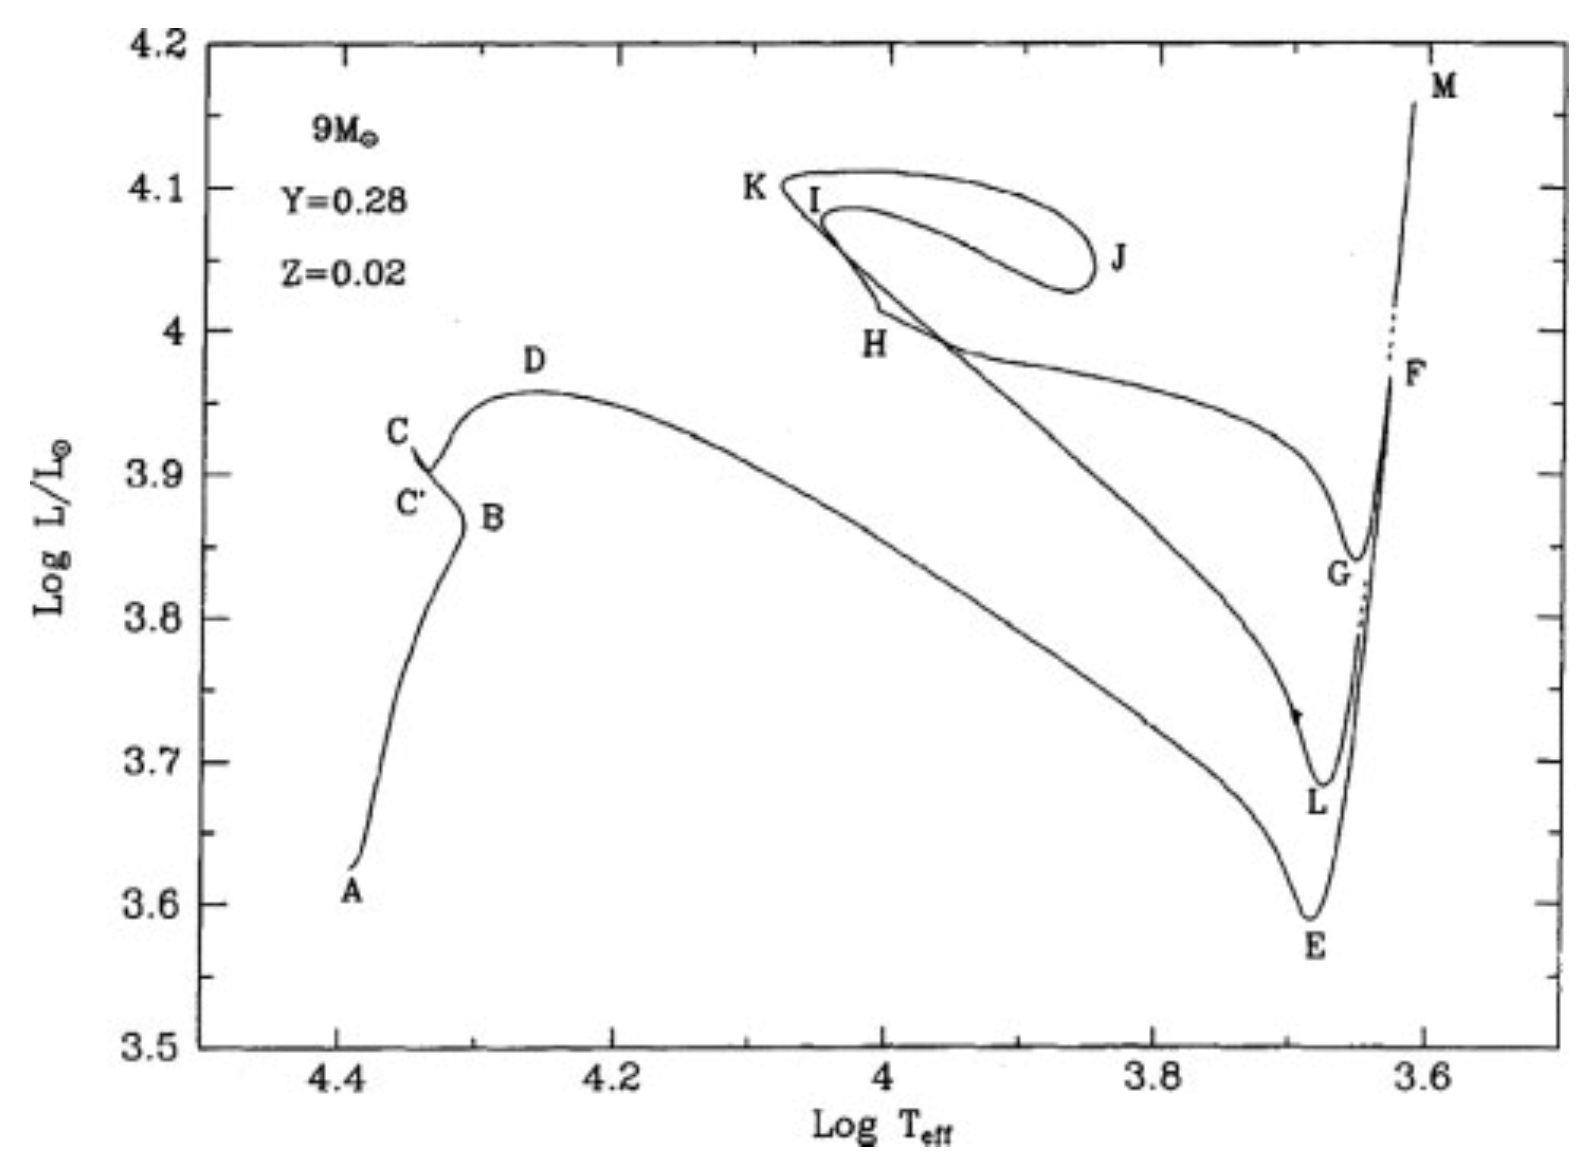
\includegraphics[width=10cm]{figures/HRD_9M.png}}
\end{figure}

{\noindent}Before disclosing what happens at points BDGHI and K (not mentioned in the previous list) it is necessary to introduce a few concepts in the language of stellar model makers. The \textbf{core} is the innermost part of the star, where nuclear reactions have greatly altered the original composition. By \textbf{envelope} one means the outer part of the star, over (most of) which nuclear burning is negligible and whose composition may still be close to the original one.

{\noindent}Next is the concept of \textbf{thermal equilibrium}. \textit{A star is said to be in thermal equilibrium (TE) when the total rate of nuclear energy generation ($L_N$) is almost perfectly equal to its surface luminosity ($L_S$).} TE means that the envelope is able to transfer outside and radiate into space quite precisely the same amount of energy which per unit time is produced by nuclear reactions in the core. If $L_S\simeq L_N$ the star is in TE and its evolution proceeds on a nuclear timescale. Conversely, if $L_S\neq L_N$ the star is out of TE, and its evolution proceeds on a thermal timescale, which usually is much shorter than the nuclear timescale. TE is often broken when the core runs out of fuel or when a new fuel is ignited. A dramatic example of breaking TE is the helium ignition in a degenerate core, called a \textbf{helium flash}. At flash peak $L_N\simeq 10^{10}\,{\rm L_\odot}$ while $L_S\simeq2000\,{\rm L_\odot}$ (and decreases!). The energy that does not escape the star is used to expand the helium core, hence relieving its degeneracy.

\begin{figure}[h]
    \floatbox[{\capbeside\thisfloatsetup{capbesideposition={right,top},capbesidewidth=4cm}}]{figure}[\FBwidth]
    {\caption{\footnotesize{The luminosity radiated from the star's surface as a function of the luminosity released by the stellar core and entering the envelope from its base, for the same track shown in Figure \ref{fig:hrd9}. Labels of relevant points along the sequence are the same as in Figure \ref{fig:hrd9}. Source: Renzini et al. (1992, Astrophys. J., 400, 280). Figure taken from Greggio \& Renzini (2011).}}
    \label{fig:lslb9}}
    {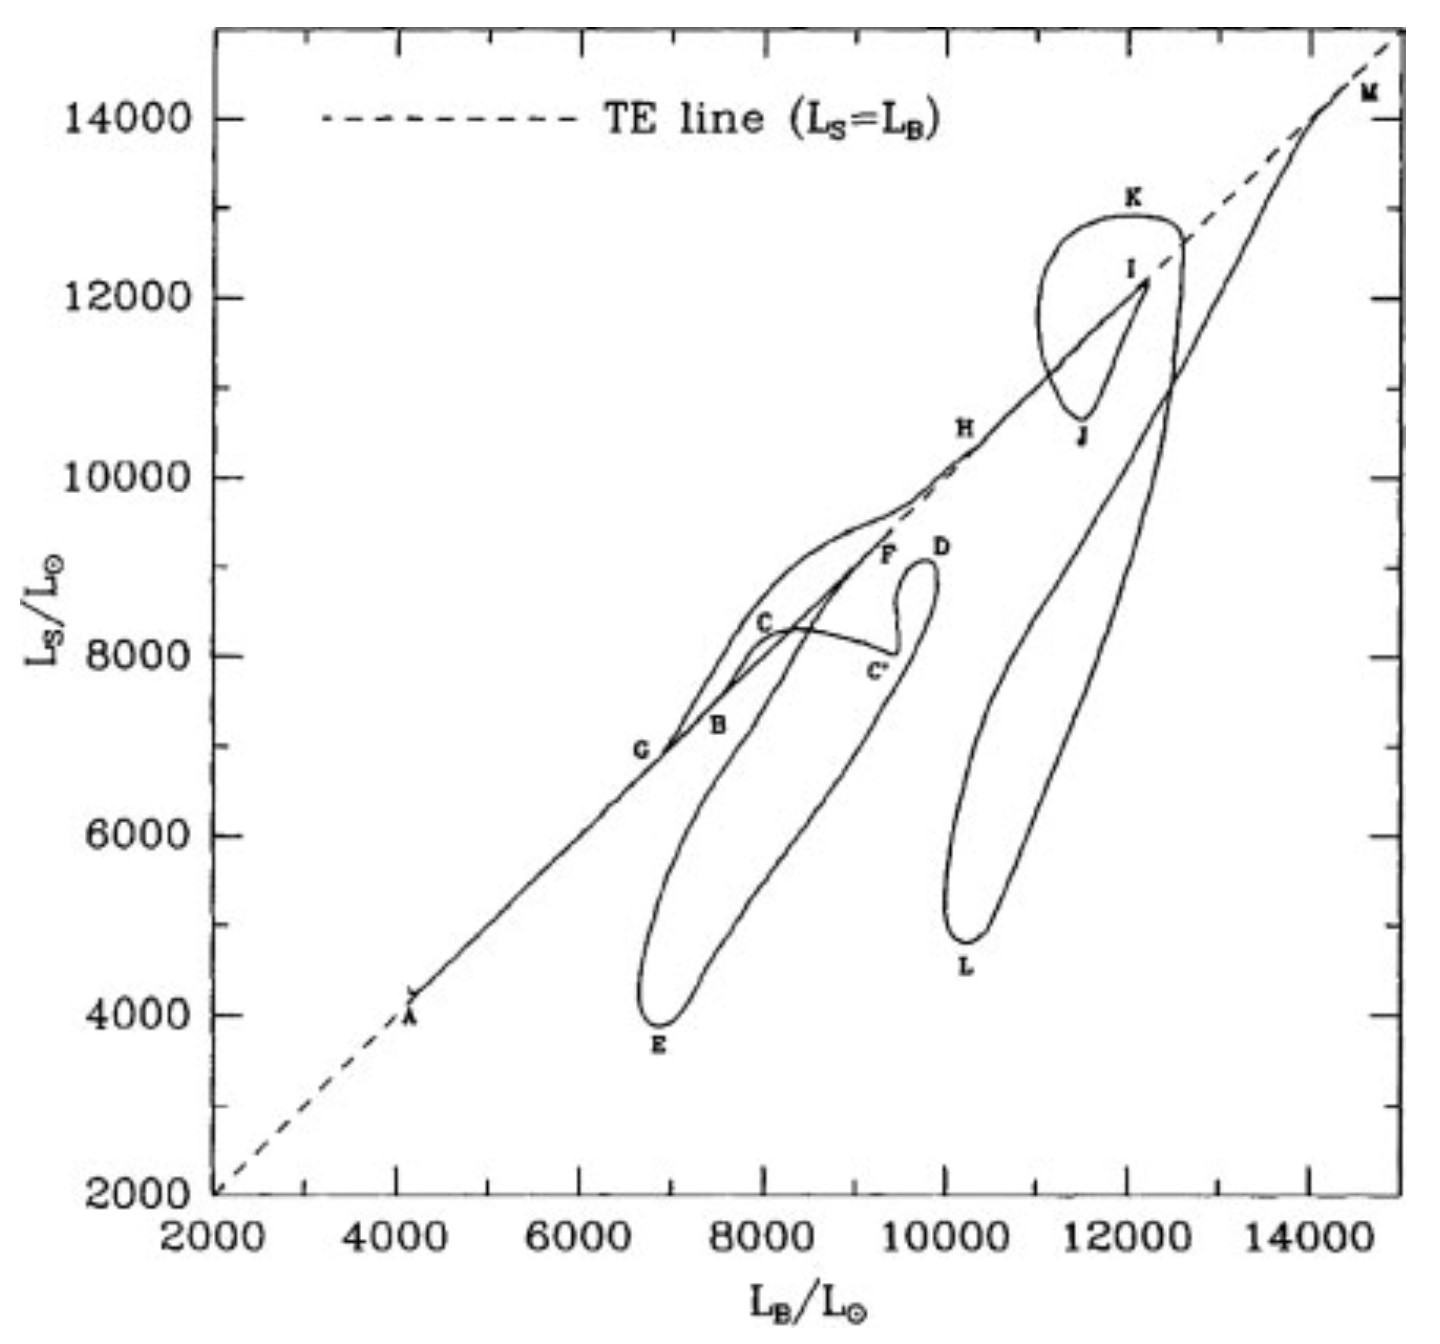
\includegraphics[width=10cm]{figures/LSLB_9M.png}}
\end{figure}

{\noindent}Evolutionary phases in TE and those out of TE can be easily identified by plotting $L_S$ versus $L_N$, or, equivalently, versus the luminosity impinging at the base of the envelope ($L_B$), as shown in Figure \ref{fig:lslb9} relative to the evolution of the same $9\,{\rm M_\odot}$ star model whose HRD is shown in Figure \ref{fig:hrd9}. Letter labels in this figure mark the same events as in Figure \ref{fig:hrd9}, so that one can identify those phases that are in TE and those which are out of it.

{\noindent}Thus, phase AB (which is most of the main sequence phase) proceeds in strict TE, but as hydrogen approaches exhaustion in the core, nuclear burning starts to fall short of keeping in pace with the rate at which energy is being radiated away, the star starts departing from TE and begins to contract (point B). At point B, as the core is running out of fuel the envelope starts losing more energy than it receives, and contracts until at point C hydrogen is effectively exhausted over the central regions, and nuclear energy generation quickly shifts to a shell surrounding a hydrogen-exhausted helium core. The quick readjustment from core to shell burning leaves the star at point C', somewhat out of TE, but then the structure tends to approach again TE, until at point D this tendency is reverted and a major excursion away from TE begins. In stars a little less massive than the one considered here, TE is actually well restored shortly after point C', and yet (as here at point D) TE is broken and stars undergo an extensive loop in the $L_S-L_B$ diagram, as shown in Figure \ref{fig:lslb9}. The journey across the HRD from point D to point E takes place on a thermal timescale, and the star expands to red giant dimensions. Clearly, a thermal instability erupts at point D. This is indeed a quite severe thermal instability, suffice to say from Figure \ref{fig:lslb9} that at the peak of the instability the core releases $\sim7000\,{\rm L_\odot}$ but the envelope radiates away only $\sim4000\,{\rm L_\odot}$, and $\sim3000\,{\rm L_\odot}$ are absorbed for its expansion.

{\noindent}The physical origin of this thermal instability is actually quite easy to understand. During phase C'D the luminosity provided by the hydrogen burning shell steadily increases as the shell moves out in the mass coordinate thanks to its own burning, and sits on a progressively more massive helium core. In response to the increasing luminosity impinging on its base ($L_B$) the envelope slowly expands. By expanding the envelope cools, and by cooling heavy metal ions begin to recombine. Besides being scattered by free electrons, photons now begin to be absorbed by such heavy ions via bound-bound and bound-free transitions: \textit{radiative opacity increases}. This opacity increase is the key factor that determines the onset of the thermal instability. At any point within the star the luminosity transmitted outwards by the radiation field is:

\begin{align*}
    L_r = 4\pi r^2 \frac{4acT^3}{3\kappa\rho} \frac{{\rm d}T}{{\rm d}r} = 4\pi r^2F_r ~ [{\rm erg\,s^{-1}}],
\end{align*}

{\noindent}where $r$ is the distance from the center, $T$ the temperature, $\rho$ the density, $\kappa$ the opacity, and $F_r$ the radiative energy flux. During phase C'D the envelope slowly expands, hence $r^2$ increases while the flux $F_r$ decreases, but their product still increases and the star is approaching TE. However, as this trend continues the increase in opacity accelerates and eventually the flux drops faster than $r^2$ increases, and their product $L_r$ starts to decrease. The decrease happens first near the stellar surface, and then (very quickly) through the whole envelope. At this point the envelope is transferring outwards and radiating away less energy than it receives from the stellar core, that is, $\Delta L=L_B-L_S>0$. But as the envelope expands more ions recombine, opacity increases further, the flux drops even more, the thermal imbalance $L_B-L_S$ increases and expansion accelerates: the stellar envelope is in a thermal runaway, as it becomes more and more unable to radiate away the energy it receives from the stellar interior.

{\noindent}At point E the surface luminosity starts to rise again, $L_B-L_S$ begins to drop, and TE is rapidly restored. What relieves the instability and saves the star from literally falling apart is convection. As the expanding envelope cools, and opacity increases, eventually the radiative gradient $\nabla_{\rm rad}$\footnote{Temperature gradients are defined as $\nabla T(\rho,T,X_i) = (\partial\log T/\partial\log P)$.} exceeds the adiabatic gradient $\nabla_{\rm ad}$, first near the photosphere, where hydrogen is only partly ionized, and then rapidly through the whole envelope. Thus, convection replaces radiative transfer in carrying out energy through the envelope, and the thermal instability is quenched since it was intimately related to the radiative mode of energy transfer. Most of the energy flux in the envelope being now carried by convective motions, the envelope ceases to absorb energy, and the surface luminosity LS starts to increase again: the star now ascends the Hayashi line, until at point F the helium burning reactions ignite in the core.

{\noindent}Following helium ignition, the helium core initiates a very slow expansion, which will last through a major fraction of the helium burning phase. This is because the helium burning core works like a breeder reactor during this stage, that is, it produces more new fuel than it burns. As \textbf{triple-$\mathbf{α}$} reactions produce fresh $^{12}$C, the $^{12}$C($\alpha,\gamma$)$^{16}$O reactions release an increasing amount of energy, and the inner core is forced to expand slightly. Such a modest expansion of the core is sufficient to cause a decrease of temperature and density in the surrounding hydrogen burning shell and the stellar luminosity correspondingly starts to decrease. The star now evolves along the \textbf{Hayashi line} from F to G, burning helium in the core and hydrogen in the shell, until thermal stability is broken again at point G. As the envelope contracts it heats up gradually, and in particular near its base, heavy ions start losing electrons. Hence opacity decreases along with the radiative gradient. As $\nabla_{\rm rad}$ drops below $\nabla_{\rm ad}$ a radiative region appears at the base of the envelope and grows outwards in mass. As this growth progresses the envelope becomes more and more transparent to radiation, until it starts radiating away more energy than it receives from the core: $L_B-L_S$ turns increasingly negative, the envelope starts deflating, but the more it contracts the more ``transparent'' it becomes, and the more energy it loses into space. The thermal instability bringing the star in its envelope deflation from point G to point H is precisely the reverse analog of the thermal instability that causes the runaway expansion from point D to point E. As envelope inflation can be ascribed to a runway recombination of heavy elements in the envelope, envelope deflation is due to a runway ionization of such heavy elements. A comparison of the three figures (Figures \ref{fig:hrd9}-\ref{fig:rvst}) helps in visualizing the onset of the thermal instability and of its results.

\begin{figure}[h]
    \floatbox[{\capbeside\thisfloatsetup{capbesideposition={right,top},capbesidewidth=4cm}}]{figure}[\FBwidth]
    {\caption{\footnotesize{The stellar radius as a function of time for the same track shown in Figure \ref{fig:hrd9}. Labels of relevant points along the sequence are the same as in Figure \ref{fig:hrd9}. Source: Renzini et al. (1992, Astrophys. J., 400, 280). Figure taken from Greggio \& Renzini (2011).}}
    \label{fig:rvst}}
    {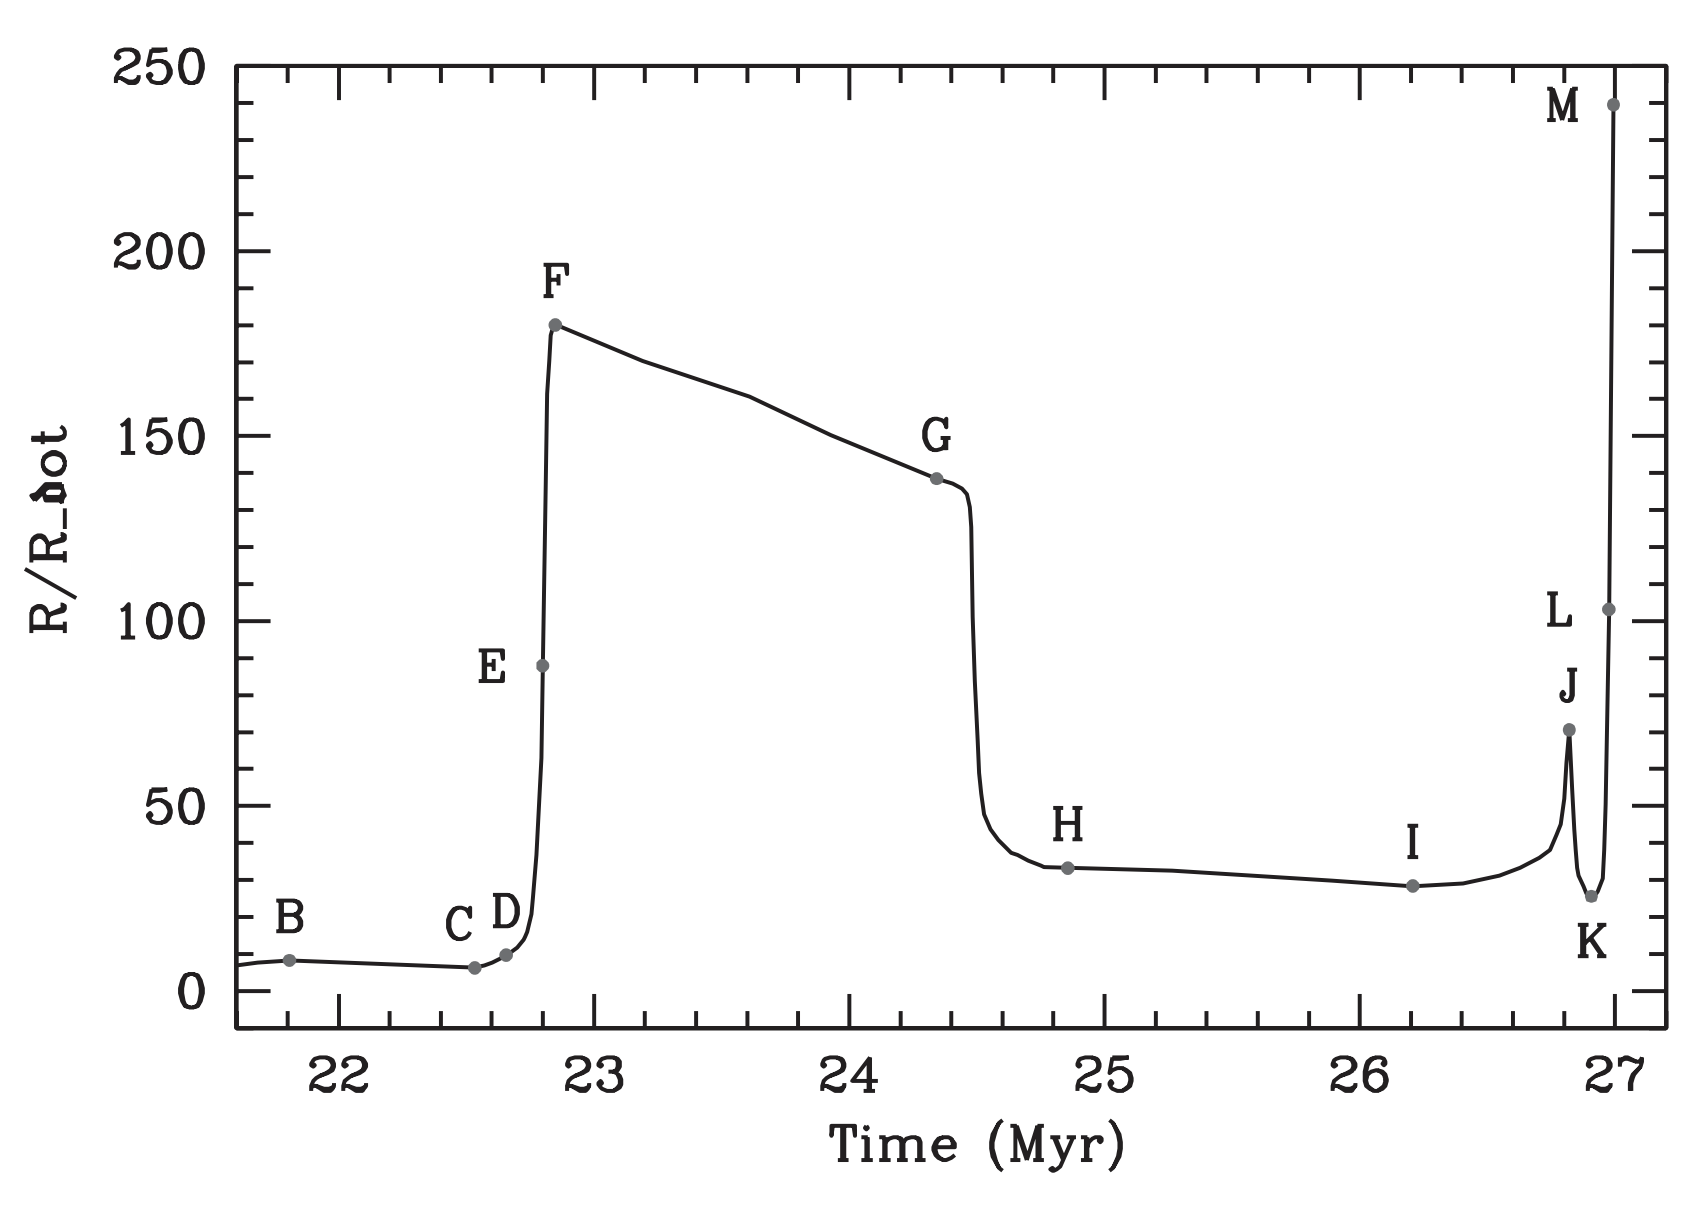
\includegraphics[width=10cm]{figures/RvsT.png}}
\end{figure}

{\noindent}Thus, in this star, the core helium burning phase in thermal equilibrium is spent in two distinct locations in the HRD: part on the Hayashi line as a red giant (F-G) and part as a blue giant (H-I) separated by a runaway contraction out of TE (G-H). This first blue loop (also called the \textbf{Cepheid blue loop}) continues after point I when TE is broken again. Here the envelope is slowly expanding in response to the slowly increasing luminosity from the core and shell burning, when the envelope turns unstable again due to the same physical process already described for the DE phase. 

{\noindent}However, the journey towards the Hayashi line is suddenly interrupted and inverted at point J, which marks the start of the so-called \textbf{second blue loop}. What happens at point J and after is a rather complex series of interconnected events: helium is exhausted in the core, the core contracts and helium burning rapidly shifts from the helium-exhausted CO core to a shell surrounding it; helium shell ignition is quite violent and causes expansion of the helium buffer above this shell: when the expansion front breaks through the hydrogen burning shell temperature and density in the shell drop; burning in the hydrogen shell (which was still providing most of the stellar luminosity) is effectively shut off completely causing a sudden drop of the luminosity impinging on the base of the envelope: $L_B$ drops below $L_S$ and the envelope stops expanding and contracts. In the meantime the strength of the helium burning shell steadily increases until it leads $L_B$ to exceed $L_S$ again, contraction stops and the star resumes at point K its runaway expansion that was temporarily stopped at J. The rest, from K to L to M is quite similar to the DEF phase, with convection replacing radiative transfer in the envelope and TE being rapidly restored, shortly before point M. Figure \ref{fig:rvst} clearly illustrates the dramatic effects of the envelope thermal instabilities on the overall structure of the star. Those phases which are in TE are nearly flat in this plot, that is, the stellar radius changes quite slowly with time. With one exception, those phases which are out of TE are instead nearly vertical, that is, the radius varies very rapidly during such runaway inflations or deflations. The exception is phase BC, which is only modestly out of TE, and contraction is relatively slow.

{\noindent}What happens past point M is still an open issue. A $9\,{\rm M_\odot}$ star lies between two domains: massive stars that eventually undergo core collapse and supernova explosion, and intermediate-mass stars, which shedding all their hydrogen-rich envelope die as a white dwarf. One believes that in a $9\,{\rm M_\odot}$ star carbon is ignited in the central core under only mildly degenerate conditions, and the star keeps ascending along the Hayashi line as a super asymptotic giant branch star experiencing a few thermal pulses in its deeper regions, where hydrogen and helium are still burning in two separate shells. Thus, if the envelope is completely lost in a wind the star leaves an ONeMg white dwarf. If instead mass loss is less severe then the core keeps growing in mass thanks to the active burning shells until electron captures in the core trigger a core collapse and we have a supernova explosion. Clearly the fate critically depends on the strength of the mass loss process.

{\noindent}\textbf{Evolution of a Solar-composition star:} Figure 1.4 shows stellar evolutionary tracks of solar composition, covering a wide range of initial masses, from a $0.8\,{\rm M_\odot}$ star, whose MS evolutionary lifetime is longer than one Hubble time, up to a $20\,{\rm M_\odot}$ model. The evolutionary tracks of stars with mass greater than $20\,{\rm M_\odot}$ are heavily affected by mass loss.

\begin{figure}[h]
    \floatbox[{\capbeside\thisfloatsetup{capbesideposition={right,top},capbesidewidth=4cm}}]{figure}[\FBwidth]
    {\caption{\footnotesize{Evolutionary tracks of solar composition star. The shaded area shows the location of low-mass ($0.55\leq M/M_\odot\leq2$) core helium burning models. Drawn using the YZVAR database (Bertelli, G. et al. 2008, Astron. Astrophys., 484, 815; 2009, Astron. Astrophys., 508, 355). Figure taken from Greggio \& Renzini (2011).}}
    \label{fig:hrdsolar}}
    {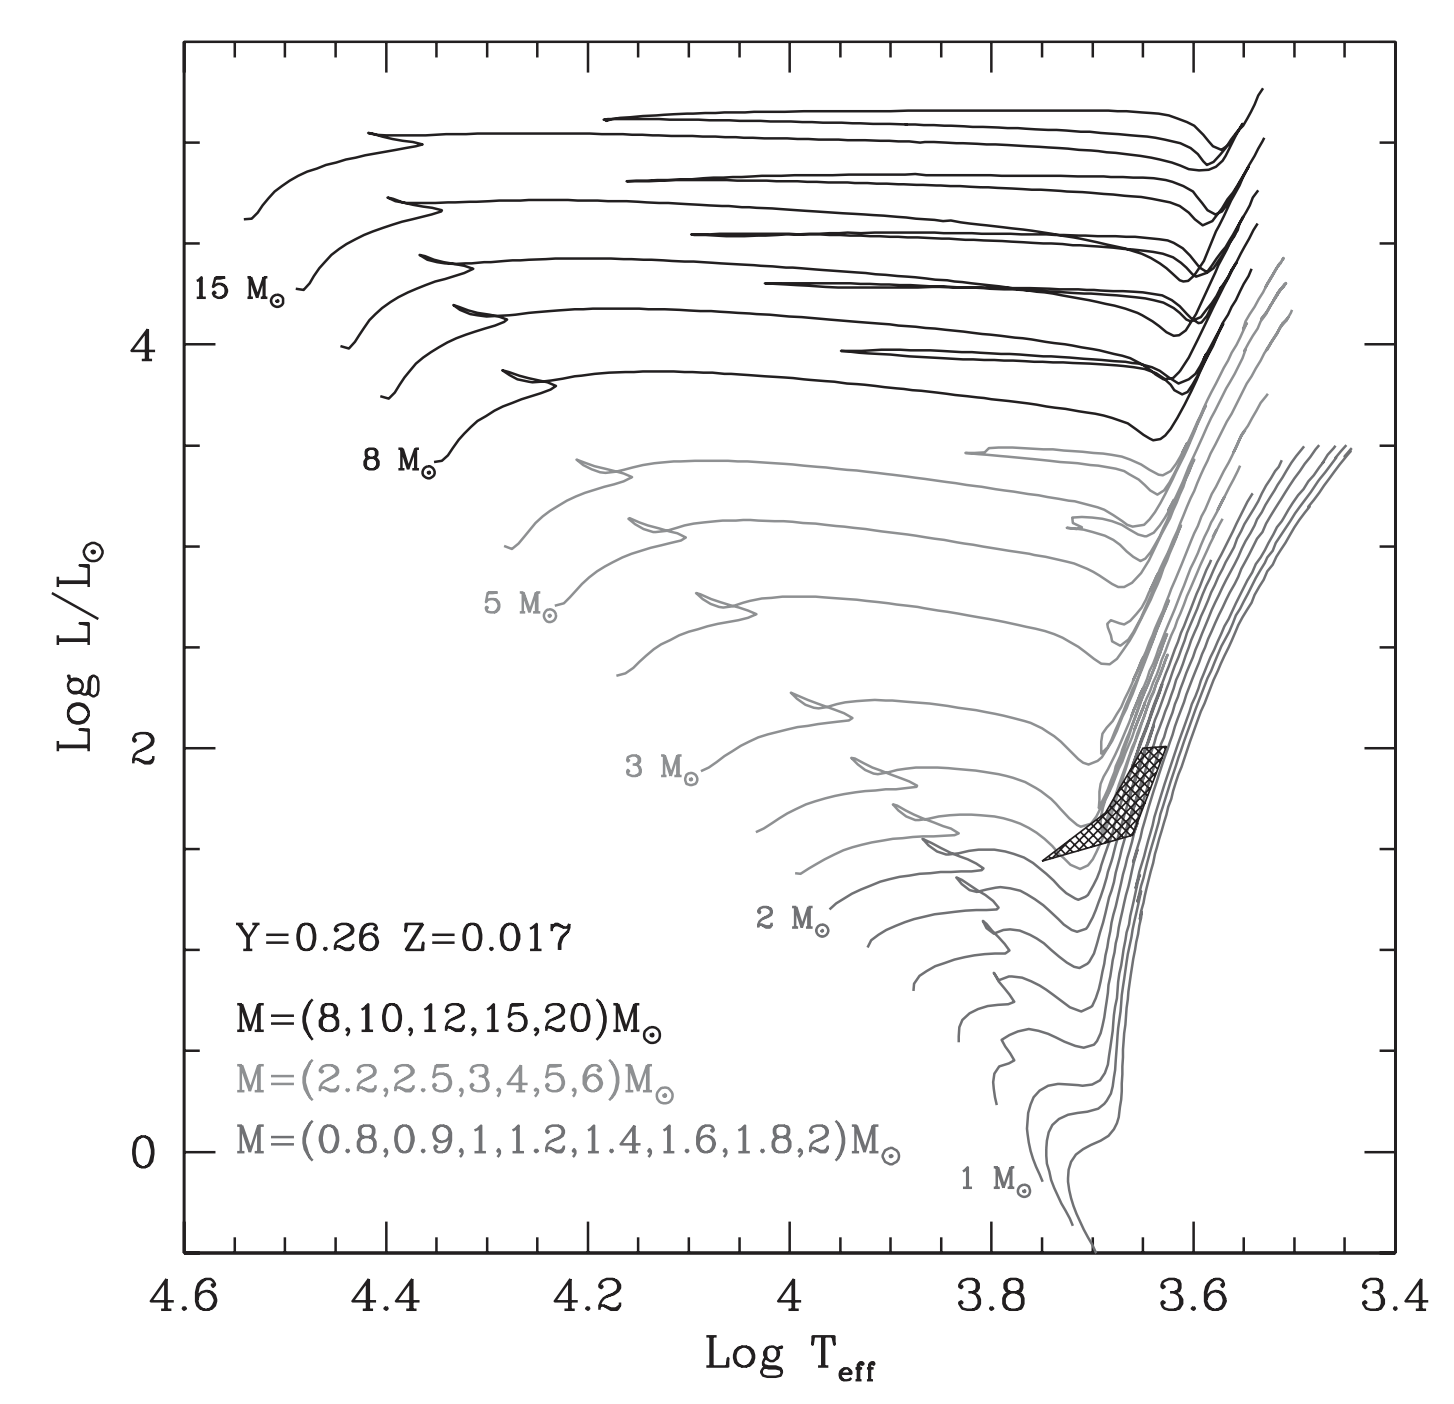
\includegraphics[width=10cm]{figures/HRD_Solar.png}}
\end{figure}

{\noindent}Different gray shades in Figure \ref{fig:hrdsolar} pertain to the different mass ranges as customarily distinguished in stellar evolution: low-mass stars, up to $\lesssim2.2\,{\rm M_\odot}$, intermediate-mass stars, up to $\lesssim8\,{\rm M_\odot}$, and high-mass stars. These ranges correspond to different physical behavior during the evolution of the stars, and the mass limits depend on chemical composition. Low-mass stars develop an \textbf{electron degenerate helium core} after their MS evolution; intermediate mass stars ignite helium under non-degenerate conditions, but develop a \textbf{CO degenerate core} after central helium burning; massive stars experience all successive nuclear burnings up to the production of an \textbf{iron core}.

{\noindent}During their MS evolution, stars with mass below $\sim1\,{\rm M_\odot}$ burn hydrogen through the \textbf{p-p chain}, whose reaction rate is not extremely sensitive to temperature, so that these stars possess a radiative core. As evolution proceeds hydrogen is progressively depleted in the inner core, more in the center than in the periphery, leading to a smooth hydrogen profile from a central minimum up to the initial abundance in the outer layers. On the HRD, the stellar track climbs to higher luminosities and temperatures until the central hydrogen is severely depleted; at this point the effective temperature starts decreasing, producing the turnoff (TO), that is, the maximum temperature point on the MS, which is easily recognizable on the CMD of globular clusters. Shortly after the TO, hydrogen is completely exhausted in the center and the hydrogen shell burning phase starts as a natural progression from the previous core hydrogen burning phase. During shell hydrogen burning, the track forms the subgiant branch (SGB), evolving at (almost) constant luminosity and decreasing temperature until the external convection penetrates deeply inside, and the star becomes almost fully convective at the base of the red giant branch (RGB).

{\noindent}The MS stars (with $M\gtrsim1\,{\rm M_\odot}$) have a convective core, since at least part of the hydrogen burning occurs through the CNO cycle, whose energy generation rate is extremely sensitive to temperature. Because of central mixing, the hydrogen profile is characterized by an inner plateau; as evolution proceeds, the extension of the convective core progressively decreases, leaving behind a gradient of hydrogen abundance. In stars with a convective core, the fuel depletion affects a sizable central region, which starts rapid contraction when approaching fuel exhaustion. This happens at the local minimum effective temperature point during the MS evolution of stars with $M>1\,{\rm M_\odot}$ (Figure \ref{fig:hrdsolar}), which signals the beginning of the overall contraction phase. The evolutionary behavior across this phase and the following runaway expansion has been already described in detail in the previous section.

{\noindent}As already mentioned, the helium core of low-mass stars is (electron) degenerate: this implies that central helium ignition is delayed because core contraction does not lead to an efficient increase of the central temperature. The (almost) fully convective star climbs along the RGB, while the hydrogen burning shell progresses outward, thereby increasing the mass of the helium core. When the core reaches a critical limit, a helium flash occurs off-center, since neutrino losses induce a temperature inversion in the innermost layers. This event in not catastrophic for the star because local expansion removes the degeneracy; instead, a sequence of flashes occurring at progressively inner locations totally remove the core degeneracy. During this phase, which lasts $1\,{\rm Myr}$, the star moves downward along the Hayashi line to settle on the core helium burning locus, either the red clump, or the horizontal branch (HB). The maximum luminosity reached on the RGB (RGB Tip, or TRGB) is a very important feature in the color-magnitude diagram (CMD) of stellar populations because it is virtually independent of mass, and then of evolutionary lifetime. This is because on the one hand the critical mass for helium ignition under degenerate conditions is almost constant ($0.5\,{\rm M_\odot}$), and on the other, along the RGB there exists a core mass-luminosity relation. The evolutionary lifetimes of low-mass stars range from $1\,{\rm Gyr}$ up to the Hubble time, as seen in Figure \ref{fig:hrdsolar}, and all of them experience the helium flash at almost the same luminosity; therefore, the CMD of a stellar population with stars older than $1\,{\rm Gyr}$ will show a prominent TRGB feature whose luminosity is known, thus allowing us to determine the distance of the stellar population. The TRGB luminosity depends slightly on metallicity, being higher for higher metal content. However, by a fortunate combination, the absolute magnitude in the I-band of the TRGB does not depend much on metallicity, for metal-poor populations. This is because the effective temperature at the TRGB also depends on metallicity: the higher $Z$, the cooler the TRGB stars, and the higher the bolometric correction (in absolute value). The trend with metallicity of the bolometric correction to the I-band largely compensates that of the tip luminosity, so that the I-band absolute magnitude of the TRGB ($M_{\rm I,TRGB}$) is almost independent of age and weakly dependent on metallicity of the parent stellar population. This makes $M_{\rm I,TRGB}$ a very effective distance indicator in galaxies.

{\noindent}The luminosity of core helium burning low-mass stars, being fixed by the mass of their hydrogen-exhausted core, is also largely independent of their total mass, thereby providing another distance indicator. However, evolution during the core helium burning phase spreads the red clump stars over $0.6$ magnitudes, as can be seen from the vertical size of the hatched region in Figure \ref{fig:hrdsolar}. In addition, the core mass at helium ignition is not a monotonic function of the total mass, and as the latter increases beyond the limit of the low-mass stars regime ($M_{\rm Hef}$), it decreases, reaches a minimum of about $0.326\,{\rm M_\odot}$, and then increases. As a result, stars with mass just above $M_{\rm Hef}$ start their core helium burning evolution at fainter luminosities, have the longest helium burning lifetimes, and cover a wider range of luminosities, compared to stars with $M<M_{\rm Hef}$. Therefore, the core helium burners of a composite stellar population with a sizable component at ages just below $1\,{\rm Gyr}$ are spread over a wide magnitude range, which limits the use of this feature for distance determinations.

{\noindent}The effective temperature of low mass core helium burning stars depends on the mass of their envelope, a dependence which is very pronounced when the envelope is thinner than for example $0.2\,{\rm M_\odot}$ for $Z\lesssim0.1\,{\rm Z_\odot}$. Below this threshold, the lower the envelope mass, the hotter the core helium burning stars. In a coeval and homogeneous stellar population the core helium burning stars all have virtually the same core mass and then luminosity; a spread of their envelope masses produces a feature on the HRD at about constant (bolometric) magnitude extending over a temperature range. The observational counterpart of this locus is the horizontal branch: a prominent feature in the HRD of globular clusters whose age is old enough to host core helium burning stars with low-mass envelopes. The existence of wide HBs in globular clusters was explained as due to a dispersion of mass lost during the RGB phase, but recently it became apparent that other effects are also at play. Evolutionary tracks during the core helium burning phase exhibit a wide variety of morphologies, depending on their mass, envelope mass, metallicity and helium abundance. At central helium exhaustion, a rapid core contraction leads to shell helium ignition; the model star expands and moves again towards the Hayashi line to start the asymptotic giant branch (AGB) evolutionary stage. However, if the envelope mass is small enough, the shell helium burning phase is entirely spent at high effective temperatures, as an AGB manqu\'e star. The hot HB stars and their AGB manqu\'e progeny are likely responsible for the UV emission from elliptical galaxies which host old stellar populations.

{\noindent}The evolution of intermediate and high-mass stars during the hydrogen and helium burning stages is very similar to what has already been described for the $9\,{\rm M_\odot}$ star. But, following helium exhaustion, intermediate-mass stars behave similarly to low-mass stars. We only notice here that for stars with mass in the vicinity of $M_{\rm Hef}$ the core helium burning phase is spent in a red clump, which becomes a wider and wider blue loop as the model mass grows. Thus, the core helium burning phase of intermediate-mass stars is spent part in the blue and part in the red. The very occurrence of the loop, its extension and the fraction of lifetime spent on each side of the loop, are sensitive to a number of parameters describing the input physics of the models, like metallicity, opacity, convection and others. Therefore, the blue-to-red ratio in stellar populations with stars in this mass range is difficult to interpret. The luminosity of intermediate mass core helium burners is instead a more robust prediction of the models, and can be effectively used as an age indicator of stellar populations.

\begin{table}[t]
    \centering
    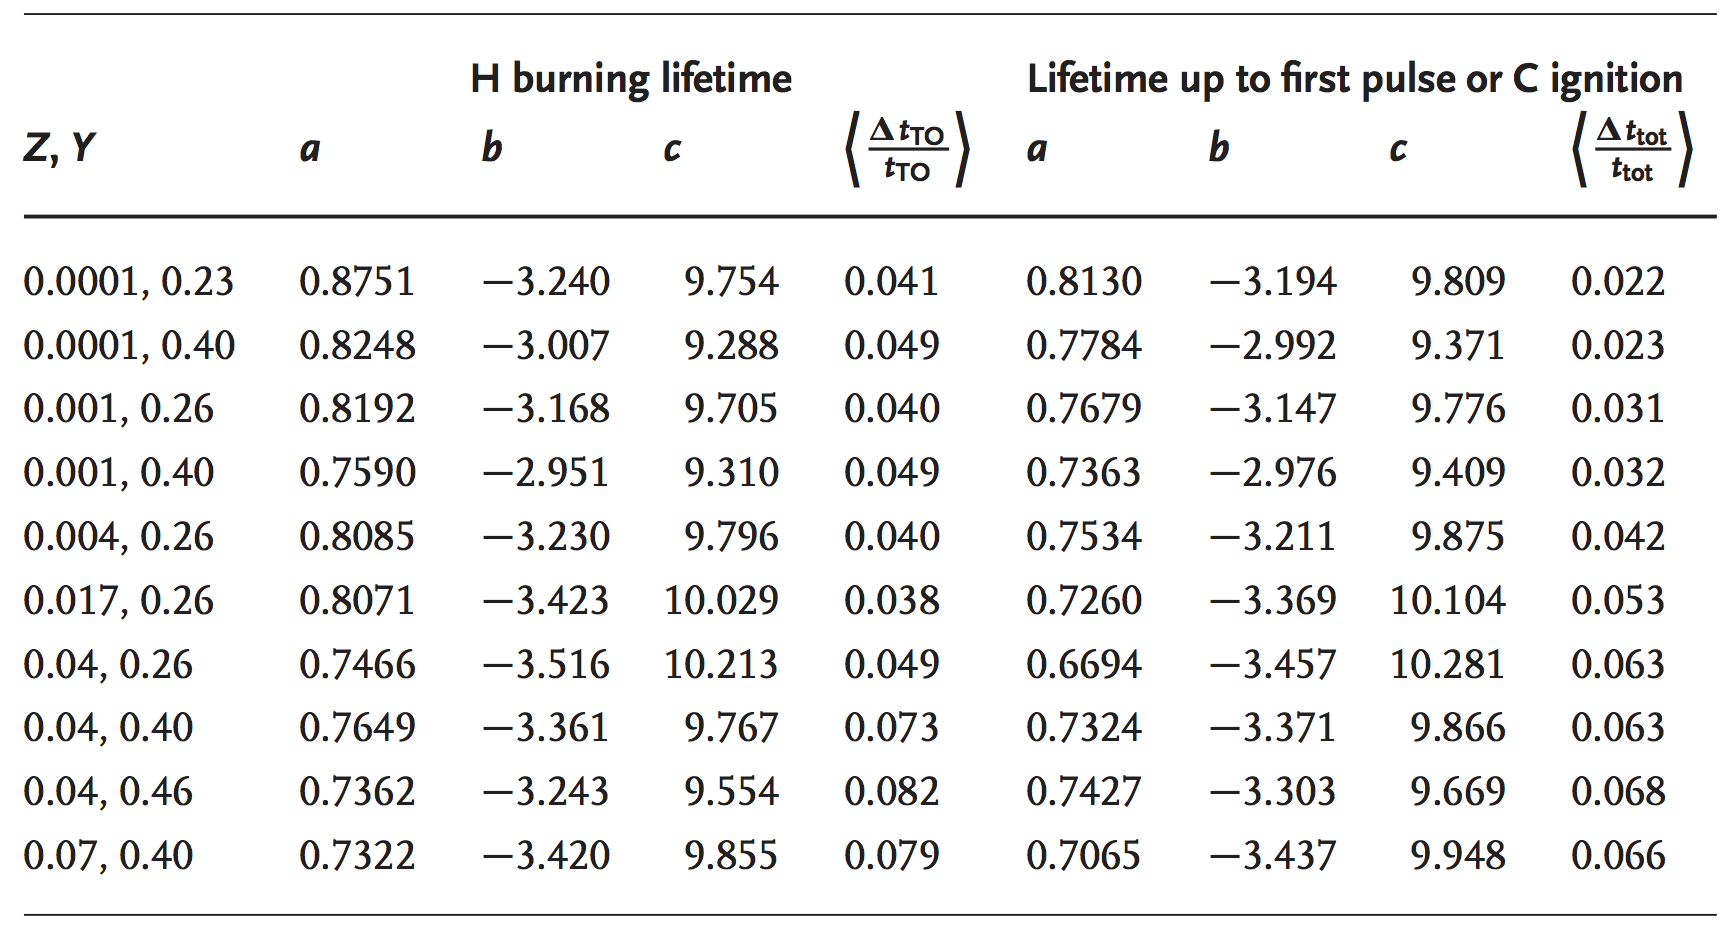
\includegraphics[width=10cm]{figures/HRD_Z_coeff.png}
    \caption{\footnotesize{Coefficients of $\log t$ for various chemical compositions, resulting from the least square fit of the hydrogen burning and the total lifetimes as a function of $M_0$. The fit covers the range $0.6\leq M_0/{\rm M_\odot} \leq20$; columns 5 and 9 report the average relative accuracy on the evolutionary lifetimes at the TO and at the first thermal pulse or central carbon ignition. The YZVAR database (Bertelli, G. et al. 2008, Astron. Astrophys., 484, 815; 2009, Astron. Astrophys., 508, 355) has been used to derive the coefficients. Table taken from Greggio \& Renzini (2011).}}
    \label{table:hrdz_coeff}
\end{table}

{\noindent}\textbf{Dependence on chemical composition:} The evolutionary tracks of given mass are very sensitive to the (initial) helium content ($Y$) and metallicity ($Z$), which control the energy generation rates and the opacity. We briefly illustrate some dependencies relevant to the interpretation of the HR diagram and of the spectral energy distribution of stellar populations.

{\noindent}At a given initial mass, evolutionary lifetimes become shorter as $Y$ increases, because stars with higher molecular weight are more compact, hotter, brighter, hence faster in consuming the hydrogen fuel, of which less is available. Instead, lifetimes become longer as $Z$ increases, because the hydrogen burning models get fainter due to the higher opacity, while the hydrogen fuel reservoir remains virtually unchanged. Table 1.2 lists the values of the coefficients of the following relation:

\begin{align*}
    \log t = a\log^2M_0 + b\log M_0 + c ~ [{\rm yr}],
\end{align*}

{\noindent}adopted to describe the evolutionary lifetimes (in years) as a function of initial mass (in ${\rm M_\odot}$). The parabolic fit over the whole considered mass range is a rather drastic approximation; nevertheless these analytic relations can be useful to estimate evolutionary lifetimes and their dependence on composition.

{\noindent}As mentioned previously, the values of mass defining the low, intermediate and high-mass range depend somewhat on chemical composition. For example $M_{\rm Hef}$ decreases with $Y$ increasing and with $Z$ decreasing. Therefore, an extended RGB on the HRD of a stellar population traces the presence of evolved stars with mass lower than $2.1\,{\rm M_\odot}$ for solar composition, or with mass lower than $1.5\,{\rm M_\odot}$ if $Z=0.001$, $Y=0.4$. However, evolutionary lifetimes at given mass also depend on composition, and, by and large, an extended and well populated RGB is developed in stellar populations older than $1\,{\rm Gyr}$ almost irrespective of chemical composition.

{\noindent}At fixed initial mass, zero age main sequence models are hotter and brighter for a higher helium content, and/or a lower metallicity. Indeed, the locus of the corresponding stars on the HRD (ZAMS) is used to infer the composition of the target stellar population, and is virtually the only way to estimate the helium content of these stars, if $Z$ is known from spectroscopy. The puzzling composition of multiple stellar populations in some galactic globular clusters has been derived from ZAMS fitting.

\begin{figure}[h]
    \floatbox[{\capbeside\thisfloatsetup{capbesideposition={right,top},capbesidewidth=4cm}}]{figure}[\FBwidth]
    {\caption{\footnotesize{a-c) Evolutionary tracks of intermediate-mass stars ($M/{\rm M_\odot}=3,4,5,6,7,8,10$) for different compositions, as labeled. In (a), the open circles mark start and the end of the core helium burning phase. Drawn using the BaSTI database (Pietrinferni, A. et al. 2004, Astrophys. J., 612, 168). the Figure taken from Greggio \& Renzini (2011).}}
    \label{fig:hrdz_int}}
    {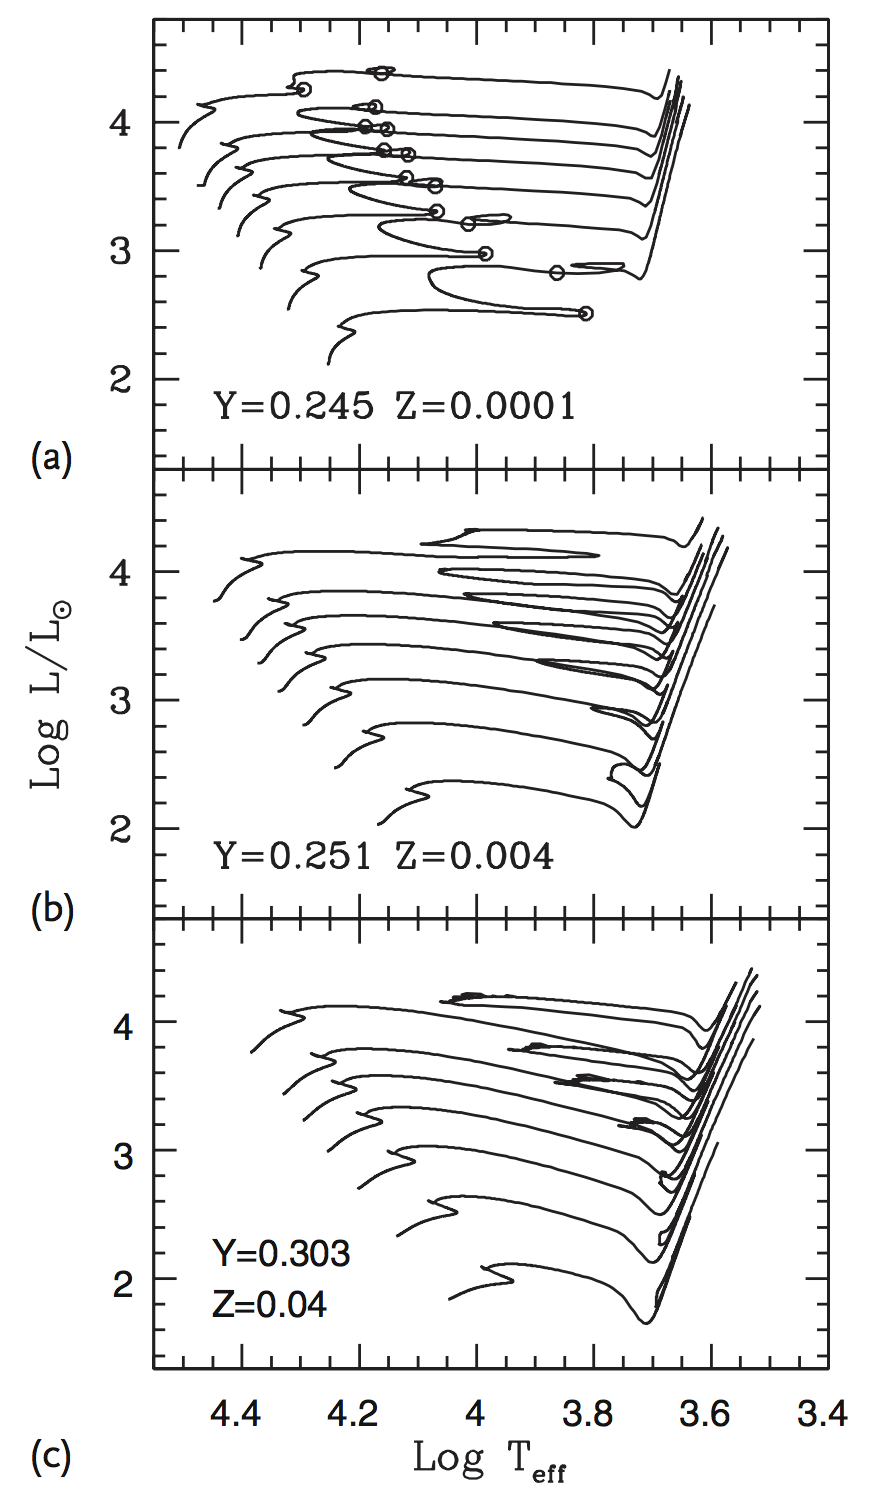
\includegraphics[width=8cm]{figures/HRD_Z_int.png}}
\end{figure}

{\noindent}Figure \ref{fig:hrdz_int} shows some evolutionary tracks of intermediate-mass stars for three different initial compositions. The described trend of the ZAMS with metal content is readily visible, together with some other properties already mentioned: at very low metallicity (Figure \ref{fig:hrdz_int}a) the entire core helium burning phase occurs in the blue part of the HRD, and the thermal runaway in the envelope which brings the model star to the Hayashi track is delayed to the very latest stages. As metallicity increases, the luminosity decrease associated with the thermal runaway gets more and more pronounced: this reflects the progressively higher opacity, and then radiative energy trapping in the envelope. At the same time, at higher metallicity it is more difficult to produce extended blue loops: the $3$ and $4\,{\rm M_\odot}$ tracks at $Z\sim2\,{\rm Z_\odot}$ do not present a blue loop at all, and the loop of the $5\,{\rm M_\odot}$ track is just alluded to. The models in Figure 1.5 are computed adopting classical recipes for the input physics, and even slight modifications of the assumptions lead to dramatic variations of the tracks shape. For example, intermediate-mass models with $Z=0.04$, $Y=0.40$ which adopt a modest overshooting from the convective core lack the loops completely, and the core helium burning phase is totally spent close to the Hayashi line.

{\noindent}Figure \ref{fig:hrdz_low} illustrates the effect of chemical composition on core helium burners of low-mass. The gray tracks in Figure \ref{fig:hrdz_low}a show that at solar composition this evolutionary phase is completely spent in the red, even for masses as low as $0.55\,{\rm M_\odot}$. Conversely, at low metallicity (black lines), low-mass core helium burners are blue, opening the possibility of producing extended HBs in old stellar populations. The tracks in Figure 1.6b show the effect of enhancing the helium abundance: at high metallicity the core helium burning phase is completely spent close to the Hayashi line for a solar helium abundance, but if the helium abundance is high, a blueward excursion occurs during the core helium burning phase which is very wide for low-mass stars. Therefore the production of blue HB stars in old stellar populations can be achieved either assuming heavy mass loss on the RGB, or a high helium content, or both. Actually, the existence of multiple stellar populations with different helium content in NGC 2808 has been first suggested on the basis of its HB stars distribution, and confirmed later from the multiple MSs. Mass loss and helium abundance have indeed an important impact on the HRD of stellar populations, as well as on their spectral energy distribution, since stars in the core helium burning phase provide an important contribution to the total light.

\begin{figure}[t]
    \centering
    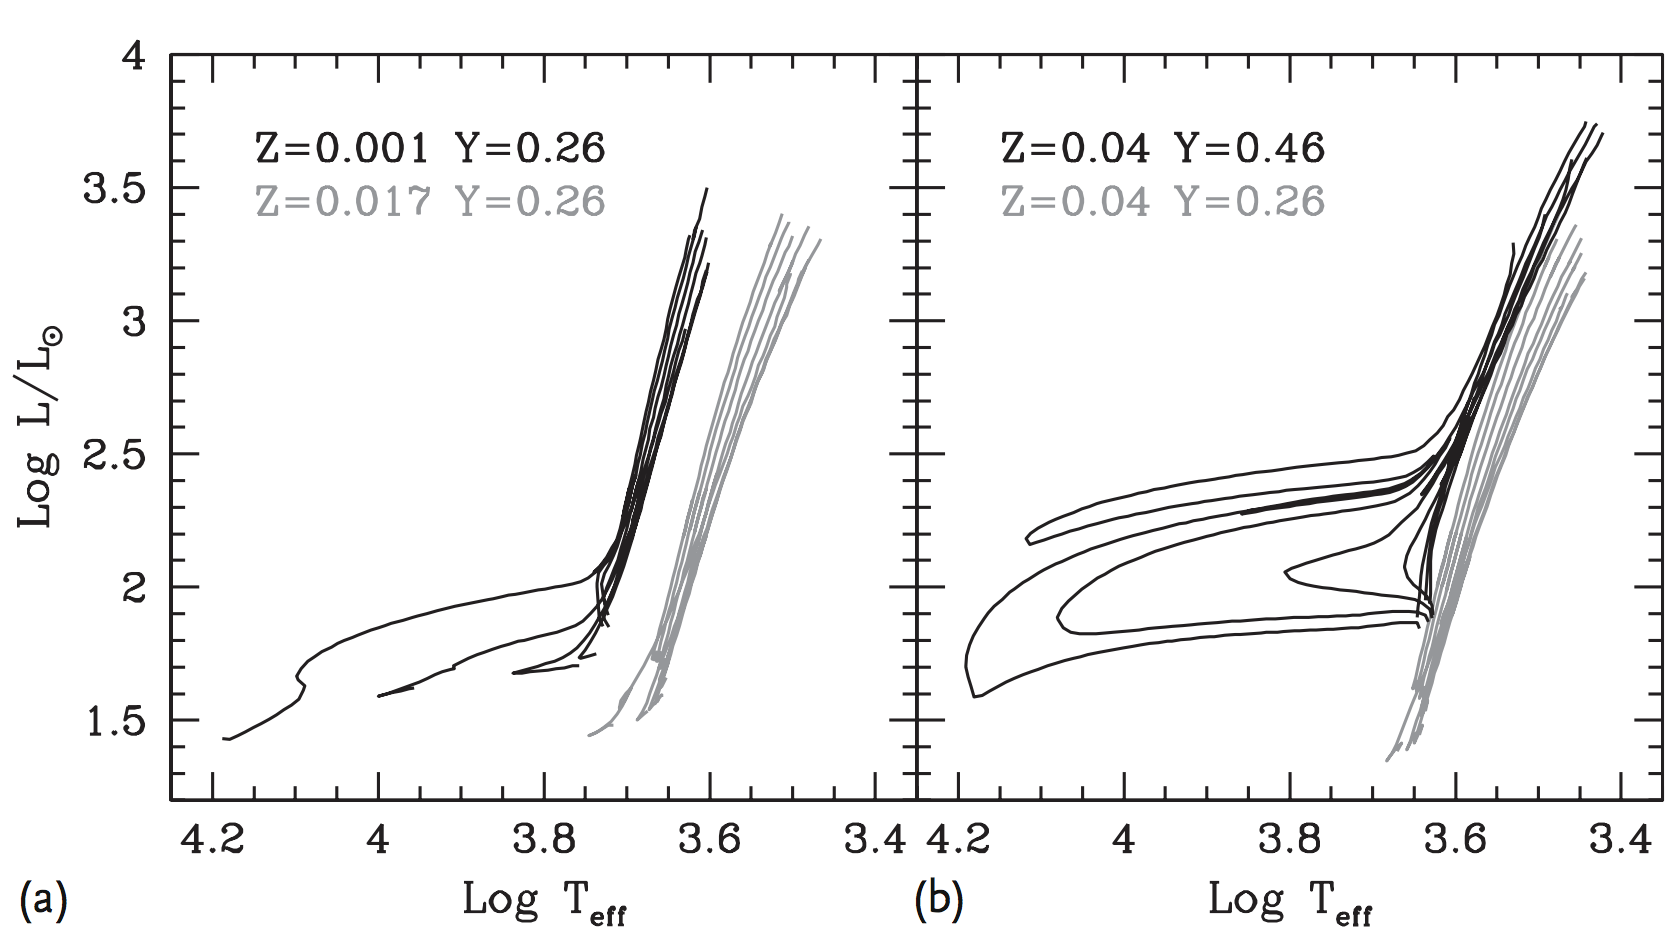
\includegraphics[width=14cm]{figures/HRD_Z_low.png}
    \caption{\footnotesize{(a,b) Evolutionary tracks of low-mass stars during the core helium burning and early AGB phases. The chemical composition is labeled. Initial model masses are $M/{\rm M_\odot}=0.55,0.6,0.65,0.7,1,1.2,1.4,1.6$ except for the ($Z=0.04,Y=0.46$) set, for which the $1.6\,{\rm M_\odot}$ track ignites helium under non-degenerate conditions. Drawn using the YZVAR database (Bertelli, G. et al. 2008, Astron. Astrophys., 484, 815; 2009, Astron. Astrophys., 508, 355). Figure taken from Greggio \& Renzini (2011).}}
    \label{fig:hrdz_low}
\end{figure}

\begin{itemize}
    \item How does metallicity affect this diagram?
    \item Elaborate on the life sequence of low-mass stars.
    \item Elaborate on the life sequence of high-mass stars.
    \item Which direction does radius increase?
    \item What's the functional form for how radius increases as a function of temperature and luminosity?
    \item Why can you use the tip of the red giant branch for distance determination?
    \item How can you use the H-R diagram to determine ages? Which of the two techniques is more accurate?
\end{itemize}

% --------------------------------------------------------------
%               2. 
% --------------------------------------------------------------

\newpage
\subsection{Question 2}

Sketch a plot of radius versus mass for various ``cold'' objects made of normal matter, including planets, brown dwarfs and white dwarfs. Explain the mass-size relationship for rocky and
gaseous objects. Why is there an upper mass limit?

\subsubsection{Short answer}

Answer.

\subsubsection{Additional context}

Additional context.

\subsubsection{Follow-up Questions}

\begin{itemize}
    \item How do you calculate the Chandrasekhar mass limit?
    \item Why is Saturn smaller than Jupiter? Or, why do we see a range of radii in extrasolar planets (e.g., hot Jupiters)?
\end{itemize}

% --------------------------------------------------------------
%               3. 
% --------------------------------------------------------------

\newpage
\subsection{Question 3}

Describe the physical conditions that lead to the formation of absorption lines in stars' spectra. What leads to emission lines?

\subsubsection{Short answer}

Answer.

\subsubsection{Additional context}

Additional context.

\subsubsection{Follow-up Questions}

\begin{itemize}
    \item Why aren't emission and absorption lines delta functions?
    \item How does this relate to population levels and excitation temperatures?
    \item Are there emission lines in the Sun? Why is there emission from the Calcium doublet?
    \item Write down the heat transfer equation. What do solutions look like?
\end{itemize}

% --------------------------------------------------------------
%               4. 
% --------------------------------------------------------------

\newpage
\subsection{Question 4}

Describe these important sources of stellar opacity: electron scattering, free-free, bound-free, and the H$^-$ ion.

\subsubsection{Short answer}

Answer.

\subsubsection{Additional context}

{\noindent}\textbf{Electron scattering:} 

{\noindent}\textbf{Free-free:} 

{\noindent}\textbf{Bound-free:} 

{\noindent}\textbf{H$^-$ ion:} Hydrogen atom has a bound state for a second electron in the field of the proton, though it has a very low ionization potential, $E_{{\rm H}^-}=0.75\,{\rm eV}$. The number density of negative hydrogen ions will be proportional to the electron density, which, in all but the most metal-poor stars, will be set by ionization of the metals (which have much lower ionization potentials that hydrogen and helium). Thus, the H$^-$ opacity will scale as $\kappa_{{\rm H}^-} \propto \rho XZ$ at low temperatures; H$^-$ is of course easily ionized at higher temperatures, and at very low temperatures even metals will not be ionized, so there will be no electrons to form H$^-$ by combining with H.

% --------------------------------------------------------------
%               5. 
% --------------------------------------------------------------

\newpage
\subsection{Question 5}

Describe the processes that can cause pulsations in a star’s luminosity, and provide at least one example of a class of stellar pulsation.

\subsubsection{Short answer}

Answer.

\subsubsection{Additional context}

Additional context.

\subsubsection{Follow-up Questions}

\begin{itemize}
    \item What about the instability strip? RR Lyrae?
    \item What is the period-luminosity relation?
    \item What is the form of the period-luminosity relation?
    \item How would you derive the time scale of pressure waves in a star?
    \item How would you order-of-magnitude estimate the period for a pulsation?
\end{itemize}

% --------------------------------------------------------------
%               6. 
% --------------------------------------------------------------

\newpage
\subsection{Question 6}

Briefly describe the sources of thermal energy for stars and planets.

\subsubsection{Short answer}

Answer.

\subsubsection{Additional context}

Additional context.

\subsubsection{Follow-up Questions}

\begin{itemize}
    \item Why do different nuclear reaction pathways have different temperature sensitivities?
    \item If I assume a constant core temperature on the main sequence, how does stellar radius depend on mass?
    \item What are some other thermal sources, like say for neutron stars?
\end{itemize}

% --------------------------------------------------------------
%               7. 
% --------------------------------------------------------------

\newpage
\subsection{Question 7}

Describe the process by which supernovae produce light. Why are Type Ia supernovae generally brighter than Type II events?

\subsubsection{Short answer}

Answer.

\subsubsection{Additional context}

Additional context.

\subsubsection{Follow-up Questions}

\begin{itemize}
    \item When a star goes supernova, how much of the luminous energy generated at the rebound is available for heating the gas? As in, where does the heat come from?
    \item Are there cases where the rebound shock wave can't blow up the star? Why, and what happens then?
\end{itemize}

% --------------------------------------------------------------
%               8. 
% --------------------------------------------------------------

\newpage
\subsection{Question 8}

Describe the condition for a star’s envelope to become convective. Why are low mass stars convective in their outer envelopes while high mass stars are convective in their inner cores?

\subsubsection{Short answer}

Answer.

\subsubsection{Additional context}

Additional context.

\subsubsection{Follow-up Questions}

\begin{itemize}
    \item How do we know that the Sun's outer envelope is convective?
    \item How far into the surface of the Sun does the convective zone permeate? How can we measure this?
\end{itemize}

% --------------------------------------------------------------
%               9. 
% --------------------------------------------------------------

\newpage
\subsection{Question 9}

What is Eddington’s luminosity limit? Explain why this limit is important for the properties and lifetimes of massive stars.

\subsubsection{Short answer}

Answer.

\subsubsection{Additional context}

Additional context.

\subsubsection{Follow-up Questions}

\begin{itemize}
    \item Draw a force diagram of what’s happening.
    \item What particles experience gravity the most?
    \item What particles experience photon pressure the most?
\end{itemize}

% --------------------------------------------------------------
%               10. 
% --------------------------------------------------------------

\newpage
\subsection{Question 10}

Explain why we know what the Sun’s central temperature ought to be, and how we know what it actually is.

\subsubsection{Short answer}

Answer.

\subsubsection{Additional context}

Additional context.

% --------------------------------------------------------------
%               11. 
% --------------------------------------------------------------

\newpage
\subsection{Question 11}

Which have higher central pressure, high-mass or low-mass main-sequence stars? Roughly, what is their mass-radius relation? Derive this.

\subsubsection{Short answer}

Answer.

\subsubsection{Additional context}

Additional context.
\subsubsection{Follow-up Questions}

\begin{itemize}
    \item How would we actually know the central pressure?
    \item What properties can we measure to test models of stellar structure?
\end{itemize}

% --------------------------------------------------------------
%               12. 
% --------------------------------------------------------------

\newpage
\subsection{Question 12}

Sketch the SED of an O, A, G, M, and T star. Give defining spectral characteristics, such as the Balmer lines and Balmer jump and Calcium doublets, and describe physically.

\subsubsection{Short answer}

Answer.

\subsubsection{Additional context}

Additional context.

\subsubsection{Follow-up Questions}

\begin{itemize}
    \item Are there emission lines?
    \item What molecular lines are in the Sun?
    \item What important lines are there are much longer wavelengths than those in the optical?
    \item What if the A star had a protoplanetary disk?
    \item What is the significance of a $\lambda$F$_\lambda$ (or $\nu$F$_\nu$) spectrum?
    \item How can the relative height of the stellar vs disk bumps change? (i.e., total energy of the system cannot change; dust bump can't be higher than star bump without extinction.)
\end{itemize}

% --------------------------------------------------------------
%               13. 
% --------------------------------------------------------------

\newpage
\subsection{Question 13}

What can be learned about young stars (T Tauri and pre-main-sequence stars) from an analysis of their spectral features?

\subsubsection{Short answer}

Answer.

\subsubsection{Additional context}

Additional context.

\subsubsection{Follow-up Questions}

\begin{itemize}
    \item How does the spectrum change as planets start to form?
\end{itemize}

% --------------------------------------------------------------
%               14. 
% --------------------------------------------------------------

\newpage
\subsection{Question 14}

Sketch the spectral energy distribution (SED) of a T Tauri star surrounded by a protoplanetary disk. How would the SED change: (a) if the disk develops a large inner hole, (b) if the dust grains in the disk grow in size by agglomeration (with the same total mass)?

\subsubsection{Short answer}

Answer.

\subsubsection{Additional context}

Additional context.

% --------------------------------------------------------------
%               15. 
% --------------------------------------------------------------

\newpage
\subsection{Question 15}

What are the primary origins of the heat lost to space by infrared luminosity of Jupiter, Earth, and Io?

\subsubsection{Short answer}

Answer.

\subsubsection{Additional context}

Additional context.

% --------------------------------------------------------------
%               16. 
% --------------------------------------------------------------

\newpage
\subsection{Question 16}

Explain the observational problem of radius inflation for hot Jupiters and describe two possible solutions.

\subsubsection{Short answer}

Answer.

\subsubsection{Additional context}

Additional context.

% --------------------------------------------------------------
%               17. 
% --------------------------------------------------------------

\newpage
\subsection{Question 17}

Explain the effects of an atmosphere on a planet’s surface temperature and the position of the “habitable zone”. What special considerations must one make for habitability around M-type stars?

\subsubsection{Short answer}

Answer.

\subsubsection{Additional context}

Additional context.

% --------------------------------------------------------------
%               18. 
% --------------------------------------------------------------

\newpage
\subsection{Question 18}

Explain the process of nuclear fusion and give two examples of important fusion processes that affect the lives of stars.

\subsubsection{Short answer}

Answer.

\subsubsection{Additional context}

Additional context.

% --------------------------------------------------------------
%               19. 
% --------------------------------------------------------------

\newpage
\subsection{Question 19}

What is Fermi’s Paradox? Explain its logic and assess the current state of the Paradox in light of modern knowledge.

\subsubsection{Short answer}

Answer.

\subsubsection{Additional context}

Additional context.

\subsubsection{Follow-up Questions}

\begin{itemize}
    \item What percentage of stars have planets?
\end{itemize}

% --------------------------------------------------------------
%               20. 
% --------------------------------------------------------------

\newpage
\subsection{Question 20}

The so-called r- and s- processes are mechanisms that produce elements heavier than iron. Describe these mechanisms and evidence for them from abundance patterns. Where is the r-process thought to act?

\subsubsection{Short answer}

Answer.

\subsubsection{Additional context}

Additional context.

% --------------------------------------------------------------
%               Resources 
% --------------------------------------------------------------

\newpage
\subsection{Resources}

\begin{itemize}
    \item Stellar Populations; Greggio \& Renzini (2011)
    \item The Fundamentals of Stellar Astrophysics, Collins (2003)
    \item Stellar Structure and Evolution, Kippenhahn, Weigert \& Weiss (2012)
    \item Evolution of Stars and Stellar Populations, Salaris \& Cassisi (2005)
    \item The Astronomical Reach of Fundamental Physics, Burrows \& Ostriker (2014)
    \item Opacity, Huebner \& Barfield (2014)
    \item Radiative Processes in Astrophysics, Rybicky \& Lightman (1979)
    \item Understanding Variable Stars, Percy (2007)
\end{itemize}

\end{document}
